\chapter{Opis projektnog zadatka}
		
		\text Cilj ovog projekta jest razviti platformu pomoću koje će se moći održavati online tečajevi. U ovo doba pandemije i izolacija, mnogi žele korisnije provesti svoje vrijeme za ekranom te naučiti neku novu vještinu. Ova aplikacija nudit će upravo to - mogućnost pohađanja tečajeva u raznim kategorijama (npr. IT, kuhanje, uređenje doma i vrta…). Tečajevi će sadržavati unaprijed pripremljene materijale poput skripti za polaznike, videosnimki i prezentacija, a unutar aplikacije postojat će i opcija konzultacija uživo putem video poziva.
		
		Pri pokretanju aplikacije, korisniku će se prikazati njen početni zaslon na kojem će moći odabrati opciju prijave s postojećim korisničkim računom ili registracije s novim korisničkim računom. Svi korisnici moraju biti registrirani kako bi mogli koristiti aplikaciju. 
		
		Neregistriranom korisniku nudi se opcija kreiranja korisničkog računa predavača ili polaznika. Jedni i drugi unose korisničko ime i lozinku za prijavu u sustav.
		
		Ukoliko se odabere opcija polaznika, korisnik mora unijeti:
		\begin{packed_item}
			\item ime
			\item prezime
			\item e-mail
			\item broj kartice za naplatu
		\end{packed_item}
	
	Ako se korisnik želi registrirati kao predavač, potrebni podaci su:
		\begin{packed_item}
			\item ime
			\item prezime
			\item e-mail
			\item IBAN
			\item \textit{opcionalno:} fotografija i kratka biografija
		\end{packed_item}
	Korisnik prijavom daje suglasnost da \textit{Bond\&Learn} prikuplja, pohranjuje, elektronički obrađuje osobne podatke za potrebe registracije i korištenja aplikacije uz poštivanje odredbi Uredbe EU o zaštiti pojedinaca u vezi s obradom osobnih podataka i o slobodnom kretanju takvih podataka te Zakona o zaštiti osobnih podataka.
	
	Svi registrirani korisnici mogu pregledavati i mijenjati svoje osobne podatke.
	
	Korisnici registrirani kao \textbf{predavač} mogu stvoriti tečaj te ga nakon toga i modificirati (dodavati materijale i ukloniti ga). Tečaj se stvara tako da se najprije odabere jedna od ponuđenih kategorija:
	\begin{packed_item}
		\item IT
		\item kuhanje
		\item uređenje doma i vrta
		\item uljepšavanje
		\item razno
	\end{packed_item}
 Nakon toga, odabire se razina zahtjevnosti tečaja koja može biti početnička, srednja ili napredna. Zatim se unosi naziv tečaja, kratki opis po želji (maksimalni kapacitet 1000 znakova) i cijena tečaja te se postavljaju materijali za učenje (PDF format do ukupno 50MB) koje je kasnije moguće dodatno uređivati. Korisnici koji prilikom registracije odaberu opciju predavača također imaju mogućnost pregledavanja polaznika svojih tečajeva te praćenja financija na pojedinom tečaju. 
	
	Korisnici koji odaberu registraciju kao \textbf{polaznik} tečaja mogu pregledavati dostupne tečajeve. Tečajeve mogu pretraživati prema kategorijama i ključnim riječima u samom nazivu tečaja. Kada pronađu tečaj koji odgovara njihovim željama i potrebama, mogu ga i upisati te, nakon uspješne naplate, pristupiti svim materijalima koje je predavač postavio dostupnima za taj tečaj. Polaznicima tečajeva dana je mogućnost slanja zahtjeva za konzultacijama, koje predavač može potvrditi i započeti ili ih otkazati.
	
	
	Jedno od sličnih rješenja jest interaktivna platforma za online učenje pod nazivom \href{https://www.coursera.org/}{\textbf{Coursera}} (slika \ref{fig:Coursera}), koja surađuje sa više od 200 svjetskih sveučilišta i kompanija. Ovo rješenje nudi 5,166 tečajeva u raznim kategorijama, no za sada ne nudi opciju kreiranja vlastitog tečaja, razvija ih isključivo u suradnji s suradnicima.
	
	\begin{figure}[H]
		
\includegraphics[scale=0.4]{slike/Coursera.PNG}
		\centering
		\caption{Naslovna stranica Coursere}
		\label{fig:Coursera}
	\end{figure}

	Drugo slično postojeće rješenje jesu online tečajevi\href{https://www.srce.unizg.hr/otvoreni-pristup-i-otvoreni-obrazovni-sadrzaji/oa-i-oer-u-srcu/srce-i-otvoreno-obrazovanje/online-tecajevi}{\textbf{Sveučilišnog računskog centra (SRCE)}}  (slika \ref{fig:SRCE}) koji nudi besplatne IT tečajeve svim korisnicima koji su registrirani na sustav za e-učenje, ali kao i prethodno rješenje ne nudi opciju stvaranja vlastitog tečaja.
	
	\begin{figure}[H]
		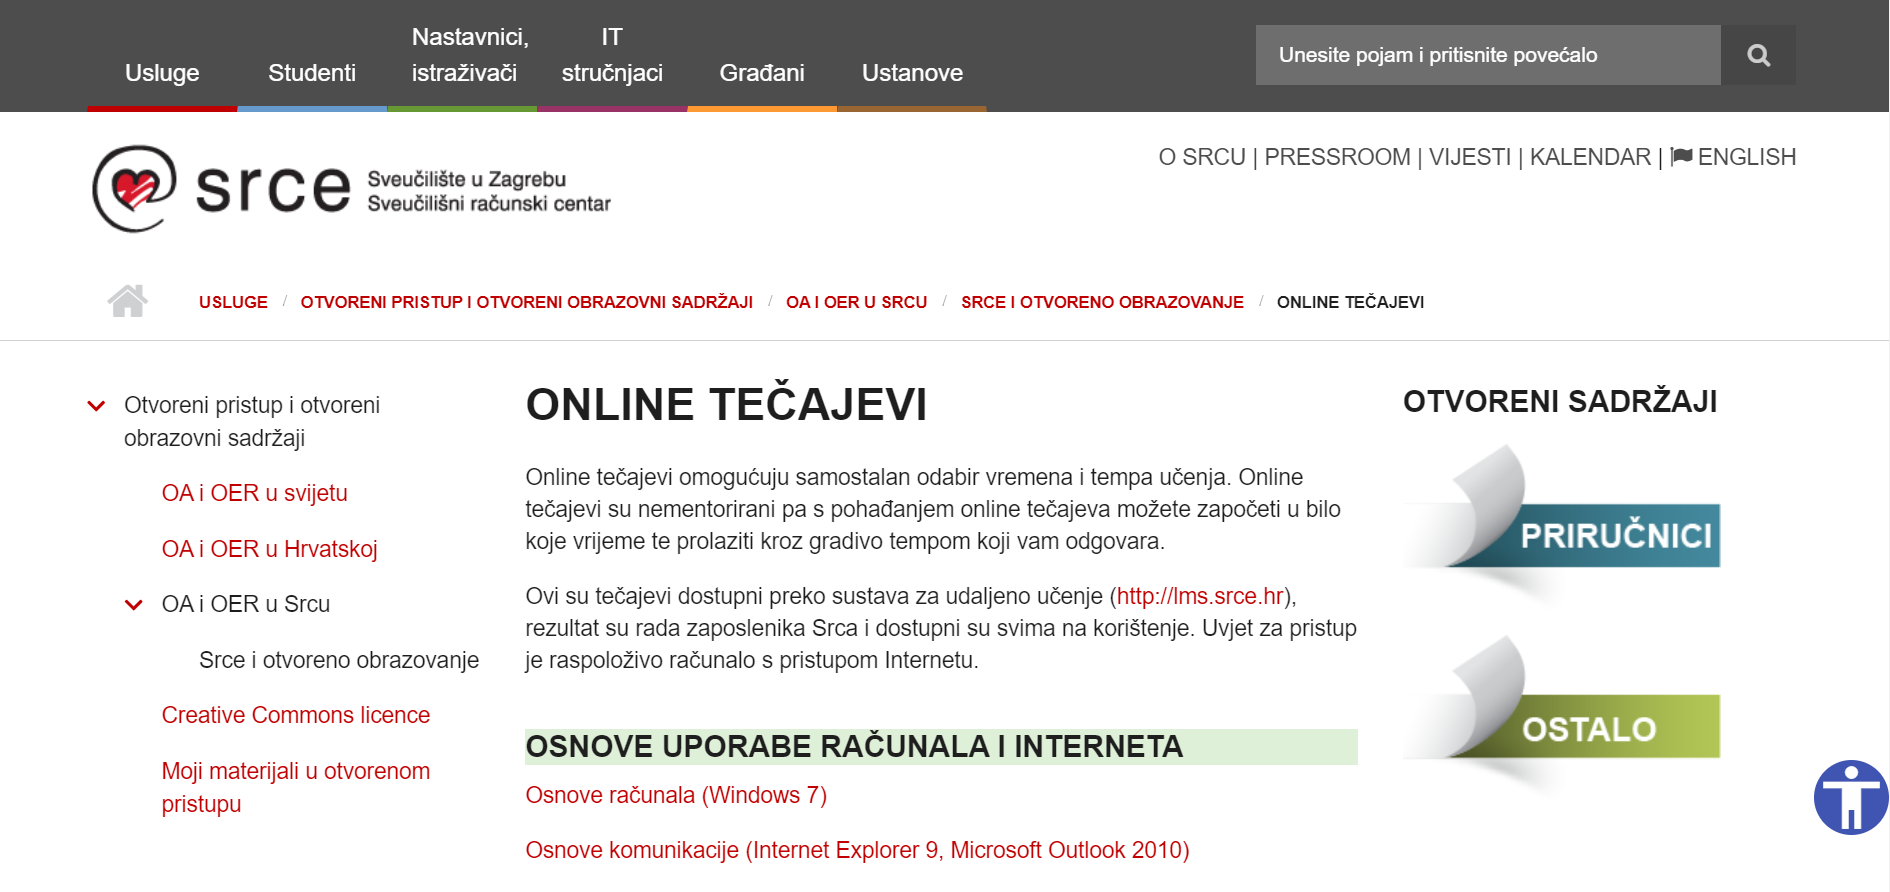
\includegraphics[scale=0.4]{slike/SRCE.PNG} 
		\centering
		\caption{Stranica online tečajeva Sveučilišnog računskog centra}
		\label{fig:SRCE}
	\end{figure}  
	
	Zadnje već postojeće rješenje koje će biti spomenuto u ovom opisu jest \href{https://www.edx.org/}{\textbf{edX}} (slika \ref{fig:edX}), platforma koja također surađuje sa preko 120 sveučilišta diljem svijeta. Nudi preko 2,500 tečajeva u 31 području interesa te je pretežito namijenjena i pogodna studentima. 
	
	\begin{figure}[H]
		
\includegraphics[scale=0.4]{slike/edX.PNG} 
		\centering
		\caption{Naslovna stranica platforme edX}
		\label{fig:edX}
	\end{figure} 

	Platforma koja se razvija na ovom projektu namijenjena je onima koji žele razviti nove vještine. Zbog velikog broja ponuđenih kategorija, ostvareno rješenje bit će od interesa široj populaciji. Jednostavan postupak stvaranja tečaja omogućit će mnogim predavačima da podijele svoje znanje sa svima zainteresiranima. Velik izbor predavača polaznicima daje mogućnost da odaberu tečaj koji najbolje odgovara njihovim željama i potrebama.
	
	Razvijenu platformu bit će moguće nadograditi. Neke od nadogradnji koje bi dodatno unaprijedile ostvareno rješenje su:
	\begin{packed_item}
		\item sustav obavijesti
		\item mogućnost dijeljenja na društvenim mrežama
		\item dodatni načini plaćanja
		\item e-mail marketing
	\end{packed_item}

		\eject
		

	